% replace all text with your own text.
% in this template few examples are mention
\chapter{Methodology}
\label{ch:method} % Label for method chapter


\section{Dataset Description}

The Kaggle heart disease dataset\cite{lapp-heart-disease-dataset-1988}, which has 1025 samples with 14 attributes each, was used in this investigation. The dataset includes a number of clinical characteristics that are frequently used to determine whether a patient has cardiac disease. Each sample has the following characteristics and represents a patient:

\begin{enumerate}
    \item Age (\textit{age}): The age of the patient in years.
    \item Sex (\textit{sex}): The gender of the patient (1 = male, 0 = female).
    \item Chest Pain Type (\textit{cp}): The type of chest pain experienced by the patient, categorized into four types: typical angina (1), atypical angina (2), non-anginal pain (3), and asymptomatic (4).
    \item Resting Blood Pressure (\textit{trestbps}): The resting blood pressure of the patient in mm Hg.
    \item Serum Cholesterol (\textit{chol}): The serum cholesterol level of the patient in mg/dl.
    \item Fasting Blood Sugar (\textit{fbs}): The fasting blood sugar level of the patient, where 1 indicates a fasting blood sugar level greater than 120 mg/dl and 0 indicates a level less than or equal to 120 mg/dl.
    \item Resting Electrocardiographic Results (\textit{restecg}): The resting electrocardiographic results of the patient, categorized into three types: normal (0), having ST-T wave abnormality (1), and showing probable or definite left ventricular hypertrophy (2).
    \item Maximum Heart Rate Achieved (\textit{thalach}): The maximum heart rate achieved by the patient.
    \item Exercise-Induced Angina (\textit{exang}): Whether the patient experienced exercise-induced angina (1 = yes, 0 = no).
    \item ST Depression Induced by Exercise Relative to Rest (\textit{oldpeak}): The ST depression induced by exercise relative to rest.
    \item Slope of the Peak Exercise ST Segment (\textit{slope}): The slope of the peak exercise ST segment, categorized into three types: upsloping (1), flat (2), and downsloping (3).
    \item Number of Major Vessels Colored by Fluoroscopy (\textit{ca}): The number of major vessels colored by fluoroscopy, ranging from 0 to 3.
    \item Thalassemia (\textit{thal}): The thalassemia status of the patient, categorized into three types: normal (3), fixed defect (6), and reversible defect (7).
    \item Target (\textit{target}): The presence of heart disease in the patient, where 1 indicates the presence of heart disease and 0 indicates the absence of heart disease.
\end{enumerate}
\subsection{Target Variable}
The target variable, \textit{target}, indicates the presence of heart disease and is binary, where 1 represents disease present and 0 represents disease not present.

\subsection{Data Types}
The dataset consists of the following features with their respective data types:
\begin{itemize}
    \item \textbf{age}: integer
    \item \textbf{sex}: integer
    \item \textbf{cp}: integer
    \item \textbf{trestbps}: integer
    \item \textbf{chol}: integer
    \item \textbf{fbs}: integer
    \item \textbf{restecg}: integer
    \item \textbf{thalach}: integer
    \item \textbf{exang}: integer
    \item \textbf{oldpeak}: float
    \item \textbf{slope}: integer
    \item \textbf{ca}: integer
    \item \textbf{thal}: integer
    \item \textbf{target}: integer
\end{itemize}




\begin{figure}
    \centering
    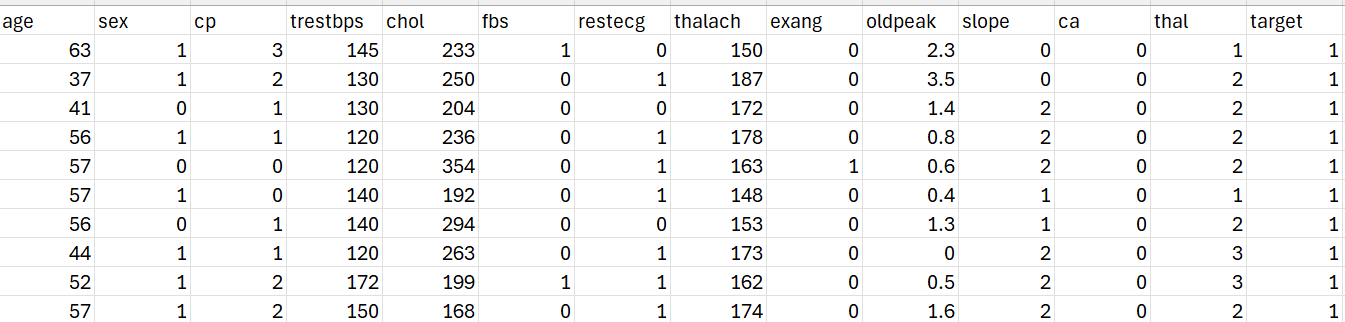
\includegraphics[width=1.0\textwidth]{figures/Datasettop10patients.png}
    \caption{Top 10 patient data from dataset}
    \label{fig:example}
\end{figure}
\section{Software Used}
The implementation and comparison of SVM and Random Forest models were performed using Python along with the following libraries:
\begin{itemize}
    \item \textbf{Python}: Python programming language was used as the primary language for coding the models.
    \item \textbf{pandas}: The pandas library was utilized for data manipulation and analysis, including reading the dataset, creating dataframes, and structuring the data.
    \item \textbf{scikit-learn (sklearn)}: The scikit-learn library was used for implementing the SVM and Random Forest algorithms, as well as for data preprocessing, model training, and evaluation.
\end{itemize}
These libraries provided the necessary tools and functions to effectively implement and compare the models, ensuring a robust and efficient analysis of the dataset.

\section{Data preparation and cleaning}
As an initial step for preparing and cleaning data in this study, a dataset comprising 1025 samples is read from a CSV file and transformed into a table using Python's pandas library. This procedure involves loading the dataset, associating the columns with their corresponding values, and constructing a table containing the samples. This process is crucial for structuring the data in an organized manner, which will simplify subsequent tasks such as data cleaning, managing missing values, and preparing the data for training and testing the SVM and Random Forest models.
\subsection{Dataset Loading and Data Type Definition}To prepare the data for analysis, I first categorized each column based on its data type. Subsequently, I imported the dataset from a CSV file into a Pandas DataFrame. This step was crucial for organizing and analyzing the data efficiently.
\begin{figure}
    \centering
    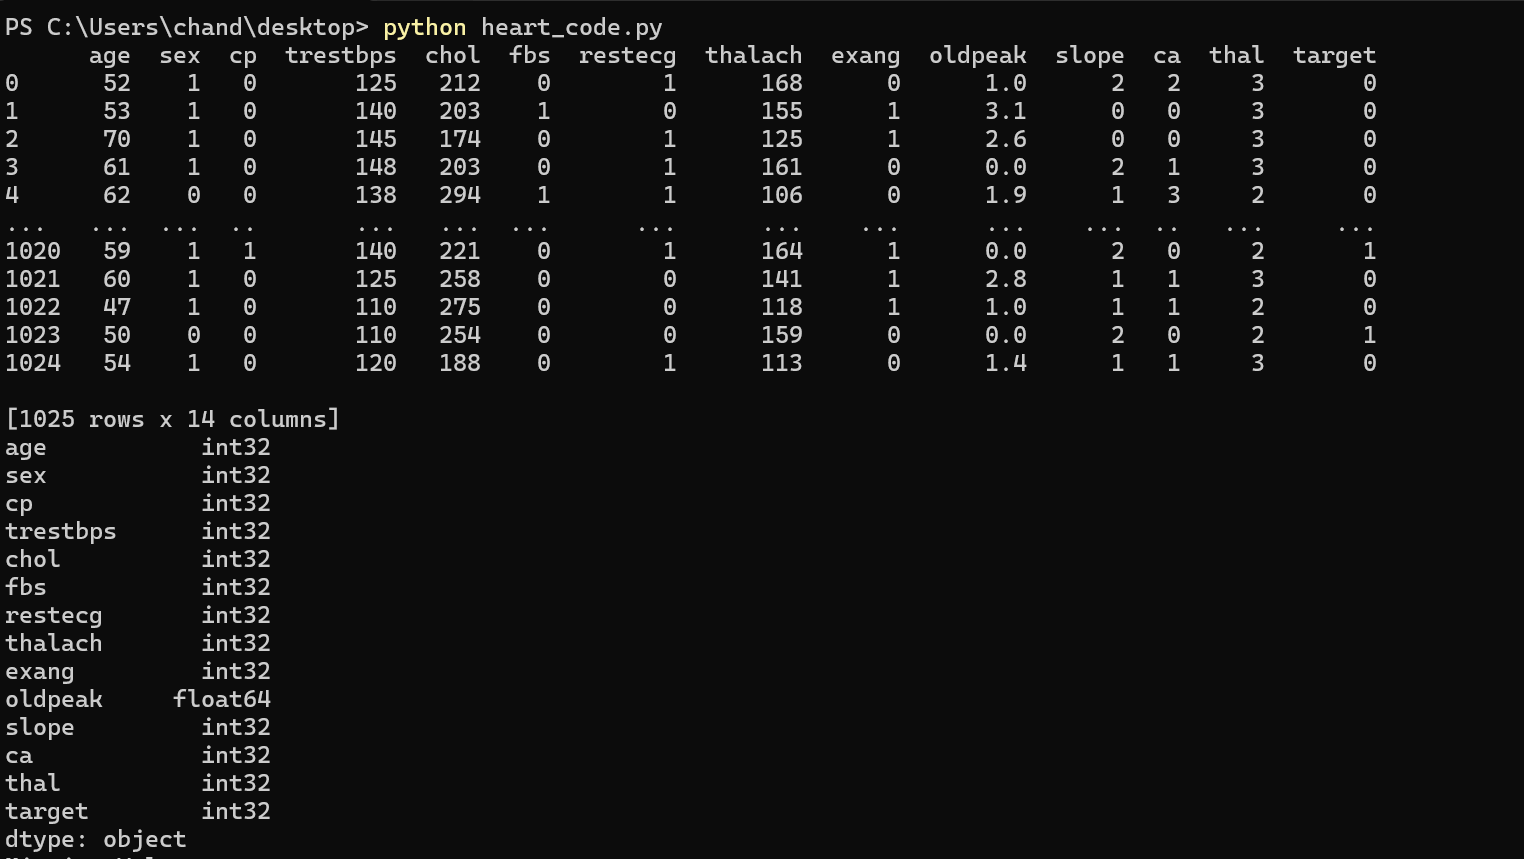
\includegraphics[width=1.0\textwidth]{figures/loaddata.png}
    \caption{Load data and data type definition}
    \label{fig:example}
\end{figure}


\subsection{Handling missing values}
Next step in our data analysis is to check for missing values in the dataset and deciding on how to handle them. We used python to inspect the dataset for missing values to analyze and found that there were 0 missing values. Consequently, no values needed to be replaced. Initially, we planned to fill any missing values with the mean, but since there were none, this step was not applicable in our data cleaning process.
\subsection{Eliminate Duplicate Values}
In the data cleaning phase, we detected and eliminated \textbf{723} duplicate entries from the dataset consisting of 1025 rows. This process was carried out using Python and the pandas library, which offers a \texttt{drop\_duplicates()} method for identifying and removing duplicate rows while preserving the first occurence of a duplicated row.

 This step is crucial as duplicate entries can distort our analysis and lead to inaccurate findings. By eliminating duplicates, we ensure the consistency and accuracy of our dataset, enhancing its reliability for subsequent data analysis and modeling endeavors.


\section{Evaluation Metrics}
\textbf{Evaluation Metrics Summary:}
\begin{itemize}
\textbf{F1 Score:} The F1 Score offers a fair evaluation of both metrics since it is the harmonic mean of Precision and Recall. Better performance is indicated by a higher value, which goes from 0 to 1. When handling skewed datasets, the F1 Score proves to be a more robust metric than Accuracy.
\[ F1 = 2 \times \frac{\text{Precision} \times \text{Recall}}{\text{Precision} + \text{Recall}} \]

\textbf{Accuracy:} The percentage of correctly predicted instances out of the total instances. It is calculated as:
\[ \text{Accuracy} = \frac{\text{Number of Correct Predictions}}{\text{Total Number of Predictions}} \times 100 \]
An overall indicator of the model's effectiveness across all classes is its accuracy. Since a high accuracy can be attained by merely projecting the majority class in every instance, it can be deceptive in situations when the classes are unbalanced. Therefore, to obtain a more comprehensive understanding of the model's performance, accuracy should be utilized in conjunction with other measures like precision and recall.
\\

\textbf{Precision:} The proportion of true positive predictions among all positive predictions. It is calculated as:
\[ \text{Precision} = \frac{\text{True Positives}}{\text{True Positives + False Positives}} \]

\textbf{Recall:} The proportion of true positive predictions among all actual positive instances. It is calculated as:
\[ \text{Recall} = \frac{\text{True Positives}}{\text{True Positives + False Negatives}} \]

\textbf{Confusion Matrix:} A table that describes the performance of a classification model. It contains four important metrics:
\[
\begin{array}{|c|c|}
\hline
\text{True Negative (TN)} & \text{False Positive (FP)} \\
\hline
\text{False Negative (FN)} & \text{True Positive (TP)} \\
\hline
\end{array}
\]
\

\section{Model Training and Testing:}

Beghdadi et al. (2020) highlight in their study how feature selection techniques, classifiers, datasets, and the training-test ratio all directly affect performance. They emphasize how crucial sample selection techniques are to guaranteeing the proper operation of the system during the testing and training phases. In order to choose samples for a stable system design, the authors advise using a stratified systematic sampling theorem.

In order to guarantee there was enough data for training and accurate assessment of the models' performance, I used a similar strategy in my research, splitting the dataset into training and testing sets using an 80-20 ratio. Better underlying pattern recognition in the data is made possible by this separation, which enhances generalization to previously unidentified data.
\begin{lstlisting}[style=mystyle, caption={Loading data, splitting dataset, and standardizing features in Python.}, label=pythoncode]
# Loading cleaned data csv file
data = pd.read_csv("cleaned_dataset.csv")

#Dataset is split into features and target
X = data.drop('target', axis=1)
y = data['target']

# 0.2 indicates 20 % data for testing and rest 80% for training the models
X_train, X_test, y_train, y_test = train_test_split(X, y, test_size=0.2)

# Standardizing the features
scaler = StandardScaler()
X_train_scaled = scaler.fit_transform(X_train)
X_test_scaled = scaler.transform(X_test)
\end{lstlisting}

The linear kernel is used in the training and testing of SVM models because it works well in situations where the data can be divided linearly, which makes it possible for the algorithm to quickly choose the best hyperplane to divide the classes. Furthermore, linear kernels frequently result in simpler models, which can be advantageous for interpretability and implementation, and are less likely to overfit, particularly in high-dimensional environments

\begin{lstlisting}[style=mystyle, caption={SVM training and testing}, label=pythoncode2]
# Train and test SVM model
svm_model = SVC(kernel='linear')
svm_model.fit(X_train_scaled, y_train)
svm_predictions = svm_model.predict(X_test_scaled)

# Evaluate SVM model
svm_accuracy = accuracy_score(y_test, svm_predictions)
svm_precision = precision_score(y_test, svm_predictions)
svm_recall = recall_score(y_test, svm_predictions)
svm_f1 = f1_score(y_test, svm_predictions)
svm_confusion_matrix = confusion_matrix(y_test, svm_predictions)
\end{lstlisting}

\begin{lstlisting}[style=mystyle, caption={Random Forest Training and Testing}, label=pythoncode3]
# Train and test Random Forest model
rf_model = RandomForestClassifier(random_state=42)
rf_model.fit(X_train, y_train)
rf_predictions = rf_model.predict(X_test)

# Evaluate Random Forest model
rf_accuracy = accuracy_score(y_test, rf_predictions)
rf_precision = precision_score(y_test, rf_predictions)
rf_recall = recall_score(y_test, rf_predictions)
rf_f1 = f1_score(y_test, rf_predictions)
rf_confusion_matrix = confusion_matrix(y_test, rf_predictions)
\end{lstlisting}






 
